\begin{enumerate}
\item 
	\begin{align}
\because
		\vec{A} - \vec{B} = \myvec{2\\3} - \myvec{4\\1} &= \myvec{-2\\2},		
\\
(\vec{A}-\vec{B})^\top (\vec{A}-\vec{B}) &= 8
	\end{align}
	Thus, the desired distance is 
	\begin{align}
		d=\norm{\vec{A}-\vec{B}} =\sqrt{8}
	\end{align}
\item 
	\begin{align}
		\vec{C} - \vec{D} = \myvec{-5\\7} - \myvec{-1\\3} &= \myvec{-4\\4}		
		\\
		\implies		(\vec{C}-\vec{D})^\top (\vec{C}-\vec{D}) &= 32
	\end{align}
Thus,	
	\begin{align}
		d=\norm{\vec{C}-\vec{D}}
 =4\sqrt{2}
\end{align}	
%	
\item 
	\begin{align}
\vec{E} - \vec{F} = \myvec{a\\b} - \myvec{-a\\-b} &= \myvec{2a\\2b}		
		\\
		\implies
		(\vec{E}-\vec{F})^\top (\vec{E}-\vec{F}) = 4a^2+4b^2 
	\end{align}
Thus,	
	\begin{align}
		d=\norm{\vec{E}-\vec{F}} =
2\sqrt{a^2+b^2}
\end{align}	
\iffalse
\begin{figure}[H]
	\begin{center} 
	    %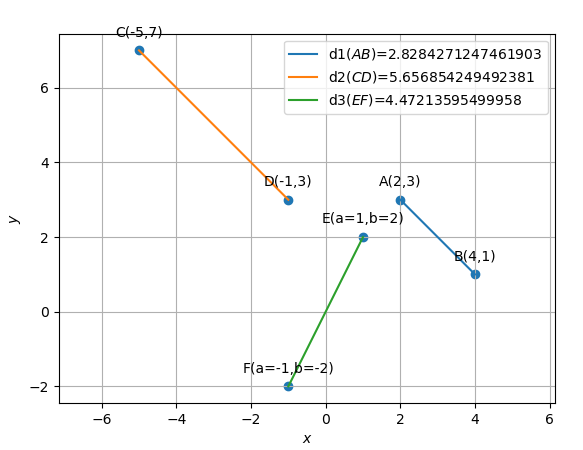
\includegraphics[width=0.75\columnwidth]{chapters/10/7/1/1/figs/graph.png}
	    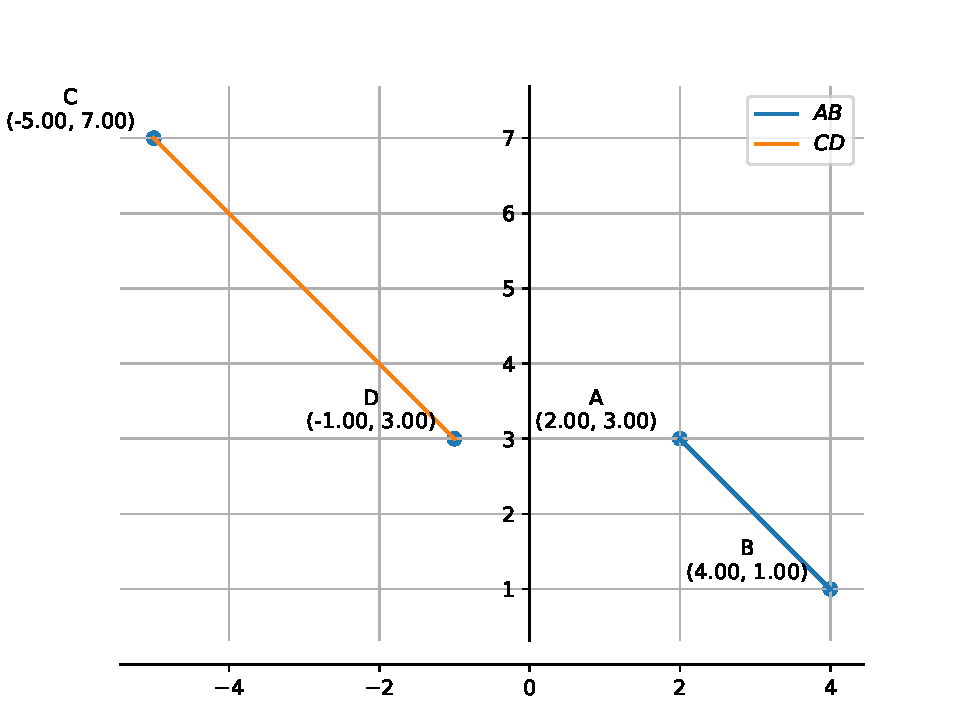
\includegraphics[width=0.75\columnwidth]{chapters/10/7/1/1/figs/fig.pdf}
	\end{center}
\caption{}
\label{fig:10/7/1/1Fig}
\end{figure}
\fi
\end{enumerate}
